\begin{figure}[htbp]
\centering
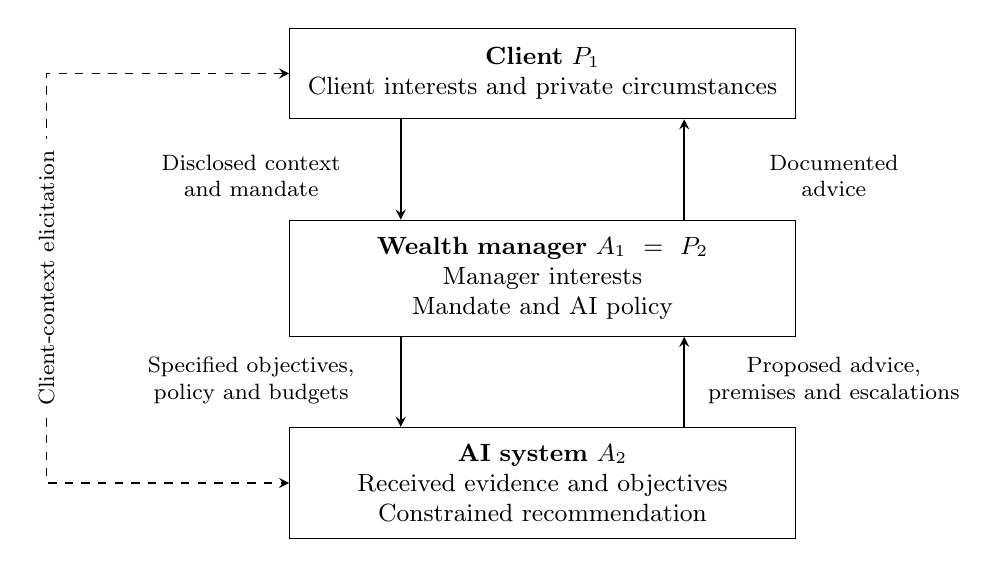
\begin{tikzpicture}[
  box/.style={draw, text width=6.0cm, minimum height=1.15cm,
    align=center, font=\small, inner sep=6pt},
  conn/.style={->, >=stealth, semithick},
  edge/.style={font=\footnotesize, align=center, text width=3.4cm},
]
\node[box] (client) at (0,0)
  {\textbf{Client $P_1$}\\Client interests and private circumstances};
\node[box] (manager) at (0,-2.6)
  {\textbf{Wealth manager $A_1=P_2$}\\Manager interests\\Mandate and AI policy};
\node[box] (system) at (0,-5.2)
  {\textbf{AI system $A_2$}\\Received evidence and objectives\\Constrained recommendation};

\draw[conn] ([xshift=-1.8cm]client.south) -- ([xshift=-1.8cm]manager.north);
\node[edge] at (-3.7,-1.3) {Disclosed context\\and mandate};
\draw[conn] ([xshift=1.8cm]manager.north) -- ([xshift=1.8cm]client.south);
\node[edge] at (3.7,-1.3) {Documented\\advice};
\draw[conn] ([xshift=-1.8cm]manager.south) -- ([xshift=-1.8cm]system.north);
\node[edge] at (-3.7,-3.9) {Specified objectives,\\policy and budgets};
\draw[conn] ([xshift=1.8cm]system.north) -- ([xshift=1.8cm]manager.south);
\node[edge] at (3.7,-3.9) {Proposed advice,\\premises and escalations};

\draw[<->, >=stealth, semithick, dashed]
  (client.west) -- (-6.3,0) -- (-6.3,-5.2) -- (system.west);
\node[font=\footnotesize, rotate=90, fill=white, inner sep=4pt]
  at (-6.3,-2.6) {Client-context elicitation};
\end{tikzpicture}
\caption{Nested delegation and client-context elicitation.}
\label{fig:nested-agency}
{\raggedright\fignote{The wealth manager acts as the client's agent ($A_1$) and the AI system's principal ($P_2$). Solid arrows show the two delegation relationships; the dashed connection shows permitted client-context elicitation. Source: the authors' conceptual model.}}
\end{figure}
